
\documentclass[12pt, a4paper]{article}

\usepackage[utf8]{inputenc}
\usepackage[T1]{fontenc}
\usepackage[russian]{babel}
\usepackage[oglav,spisok,boldsect,eqwhole,figwhole,hyperref,hyperprint,remarks,greekit]{./style/fn2kursstyle}
\graphicspath{{./style/}{./figures/}}

\usepackage{multirow}
\usepackage{supertabular}
\usepackage{multicol}
\usepackage{amsmath}
% Параметры титульного листа
\title{Решение жесткой системы\\ дифференциальных уравнений Робертсона}
\author{В.\,Г.~Пиневич}
\supervisor{А.\,В.~Котович}
\group{ФН2-61Б}
\date{2023}

% Переопределение команды \vec, чтобы векторы печатались полужирным курсивом
\renewcommand{\vec}[1]{\text{\mathversion{bold}${#1}$}}%{\bi{#1}}
\newcommand\thh[1]{\text{\mathversion{bold}${#1}$}}
%Переопределение команды нумерации перечней: точки заменяются на скобки
\renewcommand{\labelenumi}{\theenumi)}
\begin{document}

\maketitle

\tableofcontents



\newpage

\section-{Введение}
Проблема решения задачи жестких систем дифференциальных уравнений возникает во многих сферах науки и техники, в частности рассмотренная в работе задача представляет собой модель химической кинетики . Существует большое количество различных методов решения таких задач. В данной работе будет рассмотрено решение задачи Робертсона методом формул дифференцирования назад, а так же методом Адамса-Моултона.

\section{Постановка задачи}
Задача данной работы --- найти решение модели химических реакций Робертсона. 
\begin{equation}
	\label{taskDef}
	\begin{cases}
		\dot{y_1} = -0,04 y_1 + 10^4 y_2 y_3,\\
		\dot{y_2} = 0,04 y_1 - 10^4 y_2 y_3 - 3 * 10^7 y_2^2,\\
		\dot{y_3} = 3 * 10^7 y_2^2,
	\end{cases}
\end{equation}
где $t \in [0; 40]$. Начальные условия $y_1(0) = 1, y_2(0) = 0, y_3(0) = 0$.

Кроме того, требуется построить фазовые траектории решений рассмотренных методов и сделать вывод о целесообразности использования каждого из них.

\subsection{Жесткая система}
Пусть есть система дифференциальных уравнений 
\begin{equation}
	\label{example_eq}
	y_t = f(t, y), 0 \leq t \leq T, y(0) = y_0.
\end{equation}

Система называется жесткой, если для всех $t, y$ (т. е. на решениях~(\ref{example_eq})), собственные значения матрицы A удовлетворяют условиям~\cite{metoda_bmstu}. 

\begin{equation*}
	\begin{cases}
	\frac{max | Re \lambda_j |}
	{min | Re \lambda_j |} >> 1, Re \lambda_j < 0,\\
	max | Im \lambda_j | << max | Re \lambda_j |, j, k = 1, ..., J.
	\end{cases}
\end{equation*}

Схема называется абсолютно устойчивой, если $|q(\sigma)| \leq 1 $ выполняется при всех значениях~\cite{metoda_bmstu}.

Схема называется A-устойчивой, если кривая $|q(\sigma)| = 1$ лежит в правой полуплоскости $\sigma$~\cite{metoda_bmstu}. 
Когда метод А-устойчивый возможен выбор шага исключительно из соображений точности~\cite{cambridge}.

Для решения жестких задач используются абсолютно устойчивые методы, в данной работе рассмотрены многошажные неявные методы, поскольку явные методы не могут быть А-устойчивы.

\section-{Метод Адамса-Моултона}

Для схемы с двумя шагами использовалась следующая расчетная формула:

$ y_{n+2} = y_{n+1} + h \left( \frac{5}{12} f(t_{n+2},y_{n+2}) + \frac{8}{12} f(t_{n+1},y_{n+1}) - \frac{1}{12} f(t_n,y_n) \right)  $

Для решение системы алгебраических уравнений был использован метод Ньютона. Для нахождения значений в первых двух шагах использовался метод Рунге-Кутты.

\subsection{Порядок аппроксимации}

$S$-шажный метод Адамса-Моултона будет иметь порядок $s + 1$. 
Вычислим порядок согласно формуле 
\begin{equation}
	\label{approx_formula}
	p = log_2 \frac{f_i - f}{f_{i+1} - f}.
\end{equation}

Получаем следующие результаты
\begin{table}[hbt!]
	\centering
	\begin{tabular}{|l|l|l|} 
		\hline
		Шаг      & Разность     & Порядок            \\ 
		\hline
		0.1    & 1.66E-07 & 3.000227306  \\ 
		\hline
		0.05   & 2.08E-08 & 3.00011384   \\ 
		\hline
		0.025  & 2.60E-09 & 3.000061088  \\ 
		\hline
		0.0125 & 3.25E-10 &              \\
		\hline
	\end{tabular}
	\vspace*{4mm}
	\label{table-Adams-2}
	\caption{Порядки аппроксимации двухшажного метода Адамса-Моултона}
\end{table}

\subsection{Устойчивость}

Мы можем записать многошажный метода в форме
\begin{equation*}
	\sum^s_{m=0} y_{n+m} = h \sum^s_{m=0}{b_m f(t_{n+m}, y_{n+m})}, n = 0, 1...
\end{equation*}

Устойчивость численных методов для решения жестких задач определяется с помощью области абсолютной сходимости метода. Для двухшажного метода Адамса-Моултона эта область показана на графике ниже.
\begin{figure}[hbt!]
	\centering
	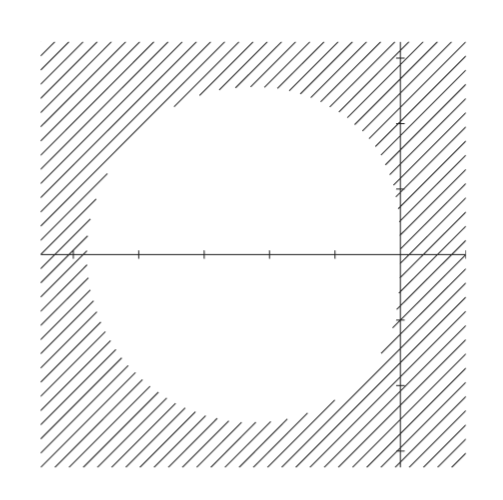
\includegraphics[width=0.5\textwidth]{lin-stab-a-m-2}%
	\caption{Область устйочивости двухшажного метода Адамса-Моултона}
	\vspace*{-2mm}
	\label{lin-stab-a-m-2}
\end{figure}

Метод Адамса-Моултона, как видно на рис.~\ref{lin-stab-a-m-2}, не является абсолютно устойчивым методом.

\section-{Метод формул дифференцирования назад}

Для схемы с двумя шагами использовалась следующая расчетная формула:

$ y_{n+2} - \tfrac43 y_{n+1} + \tfrac13 y_n = \tfrac23 h f(t_{n+2}, y_{n+2})  $

Для схемы с четырьмя шагами использовалась следующая расчетная формула:

$ y_{n+4} - \tfrac{48}{25} y_{n+3} + \tfrac{36}{25} y_{n+2} - \tfrac{16}{25} y_{n+1} + \tfrac{3}{25} y_n = \tfrac{12}{25} h f(t_{n+4}, y_{n+4}) $

Для решение системы алгебраических уравнений был использован метод Ньютона. Для нахождения значений в первых шагах использовался метод Рунге-Кутты.

\subsection{Порядок аппроксимации}

Вычислим порядок аппроксимации согласно формуле~(\ref{approx_formula})
\begin{table}[!h]
	\centering
	\begin{tabular}{|l|l|l|} 
		\hline
		Шаг      & Разность     & Порядок            \\ 
		\hline
		0.1    & 2.57E-06 & 1.948893957  \\ 
		\hline
		0.05   & 7.36E-07 & 1.911532203  \\ 
		\hline
		0.025  & 1.96E-07 & 1.957753587  \\ 
		\hline
		0.0125 & 5.04E-08 &              \\
		\hline
	\end{tabular}
	\vspace*{4mm}
	\label{table-BDF-2}
	\caption{Порядки аппроксимации метода BDF-2}
\end{table}

\begin{table}[!h]
	\centering
	\begin{tabular}{|l|l|l|} 
		\hline
		Шаг      & Разность     & Порядок \\        \hline
		0.1    & 1.27E-10 & 3.926687816  \\ 
		\hline
		0.05   & 1.02E-11 & 3.994735551  \\ 
		\hline
		0.025  & 7.06E-13 & 3.929859553  \\ 
		\hline
		0.0125 & 4.64E-14 &              \\
		\hline
	\end{tabular}
	\vspace*{4mm}
	\label{table-BDF-4}
	\caption{Порядки аппроксимации метода BDF-4}
\end{table}

\newpage

\subsection{Устойчивость}

Можно показать, что для порядков 1 и 2 BDF методы А-устойчивы, а для порядков от 3 до 6 область абсолютной устойчивости становится меньше по мере увеличения порядка. При порядке больше 7 и более размер области абсолютной сходимости недостаточен для решения жестких задач. Более подробно это описано в работах Gear (1971, раздел 11) и Lambert (1973, раздел 8).

Устойчивость численных методов для решения жестких задач определяется с помощью области абсолютной сходимости метода. Для методов BDF эти области показаны на графиках ниже.

\begin{figure}[!h]
	\centering
	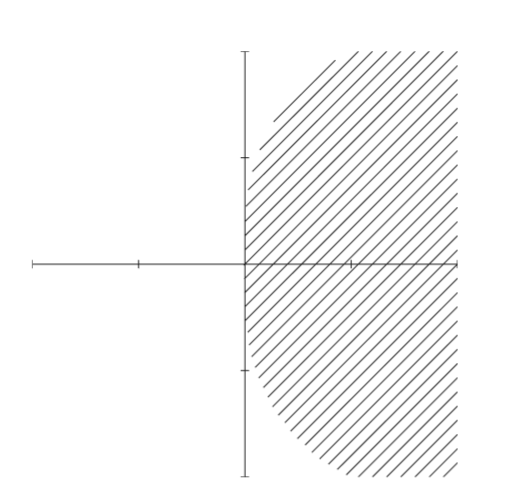
\includegraphics[width=0.5\textwidth]{lin-stab-bdf-2}%
	\caption{Область устйочивости метода BDF-2}
	\vspace*{-2mm}
	\label{ser_graph}
\end{figure}

\begin{figure}[!h]
	\centering
	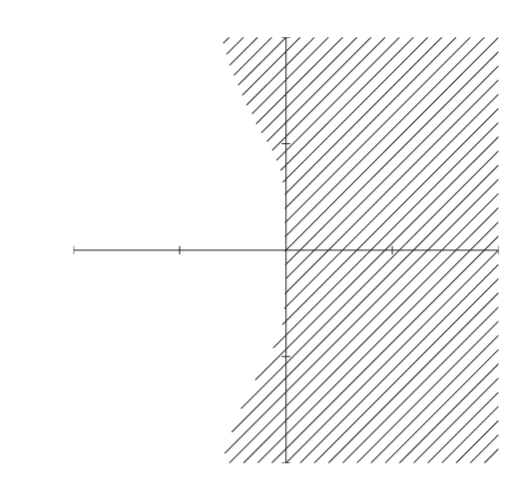
\includegraphics[width=0.5\textwidth]{lin-stab-bdf-4}%
	\caption{Область устйочивости метода BDF-4}
	\vspace*{-2mm}
	\label{ser_graph}
\end{figure}

BDF-2 метод является А-устойчивым~\cite{cambridge}.
Согласно второму барьеру Далквиста наибольший порядок многошажного метода второй.
В идеале область сходимости должена включать в себя левую половину комплексной плоскости и в таком случае метод будет считаться А-устойчивым. Однако методы BDF с порядком больше двух не могут быть А-устойчивыми. Но область устойчивости методов высокого порядка включает в себя большую часть левой полуплоскости и в частности всю отрицательную действительную ось. BDF методы являются наиболее эффективными линейными многошаговыми методами такого типа~\cite{cambridge}.

Метод считается $A(\alpha)$ устойчивым для $\alpha \in [0, \pi / 2]$, если клин
\begin{equation*}
	\nu_\alpha = \{ \rho e^{i \theta}: \rho > 0, | \theta + \pi | < \alpha \}
\end{equation*}
содержится в области абсолютной устойчивости. Другими словами, если все собственные числа системы уравнений находятся в области $\nu_\alpha$, то уменьшение шага из-за ограничений устойчивости не требуется.


\section-{Результаты}

\newpage
\section-{Заключение}
 
\newpage
\begin{thebibliography}{2}
\bibitem{metoda_bmstu} Холодов А., Лобанов А., Евдокимов А. Разностные схемы для решения жестких обыкновенных дифференциальных уравнений в пространстве неопределенных коэффициентов, М.: Московский физико-технический институт, 2001. --- 48~с.
\bibitem{cambridge} Iserles A. A First Course in
the Numerical Analysis
of Differential Equations, М.: Изд-во Cambridge University Press, 2009. --- 481 с.
\bibitem{iowa} Atkinson, Kendal E. An introduction to numericlal analysis, М.: Изд-во John Wiley \& Sons, 1988 --- 663~с.
\bibitem{haier} Хайер Э., Ваннер Г. Решение обыкновенных дифференциальных уравнений. Жесткие и дифференциально-алгебраические задачи. Пер. с англ., М.: Изд-во Мир, 1999. --- 685~с.

\end{thebibliography}

\end{document} 